\documentclass[10pt,journal,compsoc]{IEEEtran}

\usepackage{graphicx}
\usepackage{multirow}
\usepackage{amsmath,amssymb,amsfonts}
\usepackage{amsthm}
\usepackage{mathrsfs}
\usepackage{xcolor}
\usepackage{booktabs}
\usepackage{algorithm}
\usepackage{algorithmicx}
\usepackage{algpseudocode}
\usepackage{cite}
\usepackage{tikz}
\usetikzlibrary{shapes.geometric, arrows, positioning, fit, calc}

\newtheorem{theorem}{Theorem}
\newtheorem{lemma}{Lemma}
\newtheorem{definition}{Definition}

\begin{document}

\title{Verifiable and Pairing-Free Certificateless Searchable Encryption with Complete Keyword-Guessing Attack Resistance}

\author{Mohammed~Wasim~Khan
\IEEEcompsocitemizethanks{\IEEEcompsocthanksitem M. W. Khan is with the Department of Computer Science. E-mail: wasim@example.com.}
}

\IEEEtitleabstractindextext{%
\begin{abstract}
The rapid proliferation of Mobile and Medical Internet of Things (MIoT) has driven the adoption of cloud servers for outsourced data storage. However, preserving data privacy while maintaining searchability remains a critical challenge. Certificateless Searchable Encryption (CL-SE) eliminates the certificate management overhead of traditional PKI and the key escrow problem of Identity-Based Cryptography. Yet, existing CL-SE schemes suffer from three major limitations: (1) heavy reliance on computationally expensive bilinear pairings; (2) vulnerability to Outside Keyword-Guessing Attacks (OKGA) when trapdoors are intercepted; and (3) a lack of verifiable search mechanisms, forcing users to blindly trust that the ``honest-but-curious'' cloud server has returned complete results. In this paper, we propose a novel pairing-free, verifiable certificateless searchable encryption scheme designed for IoT-cloud environments. The proposed scheme achieves simultaneous resistance against both Inside and Outside Keyword-Guessing Attacks (IKGA/OKGA) through a server-bound trapdoor blinding mechanism. Furthermore, we integrate a Merkle Hash Tree (MHT) structure to guarantee search completeness and soundness. Formal security proofs in the random oracle model demonstrate that the scheme's security reduces to the hard Computational Diffie-Hellman (CDH) problem. Theoretical performance analysis and experimental simulations confirm that the proposed pairing-free construction is highly efficient and scalable, making it ideally suited for deployment in resource-constrained MIoT networks.
\end{abstract}

\begin{IEEEkeywords}
Searchable Encryption, Certificateless Cryptography, Keyword Guessing Attacks, Verifiable Search, Internet of Things, Merkle Hash Tree
\end{IEEEkeywords}}

\maketitle
\IEEEdisplaynontitleabstractindextext
\IEEEpeerreviewmaketitle

\section{Introduction}\label{sec:intro}

\IEEEPARstart{T}{he} integration of Internet of Things (IoT) devices with cloud computing paradigms has revolutionized data processing, particularly in domains such as electronic healthcare and smart cities. Because IoT devices possess limited storage and computational capacity, outsourcing encrypted data to external cloud servers has become standard practice. However, outsourcing introduces severe privacy concerns. To retrieve specific files without decrypting the entire database, Searchable Encryption (SE) was introduced, allowing a cloud server to test encrypted keywords against encrypted trapdoors. 

While early Public Key Encryption with Keyword Search (PEKS) schemes relied on traditional Public Key Infrastructure (PKI), the burden of managing and revoking digital certificates is prohibitively expensive for IoT networks. Identity-Based SE (IB-SE) resolved certificate management but introduced the key escrow problem, where a central Private Key Generator knows all user keys. Certificateless Searchable Encryption (CL-SE) solves both issues by splitting the private key between a Key Generation Center (KGC) and the user.

\subsection{Research Gap and Problem Statement}
Despite the architectural advantages of CL-SE, deploying current schemes in dynamic IoT environments presents three unsolved challenges, which represent the core research gap addressed in this paper:

\subsubsection{The Computational Bottleneck of Pairings}
The vast majority of existing CL-SE schemes \cite{lu2023certificateless, elhabob2020efficient} rely heavily on bilinear pairing operations over elliptic curves to establish shared secrets during the search phase. Bilinear pairings are notoriously resource-intensive, requiring significantly more clock cycles than standard scalar multiplication. In resource-constrained environments like Mobile IoT (MIoT), this computational overhead results in unacceptable latency and severe battery drain.

\subsubsection{The Keyword Guessing Attack (KGA) Vulnerability}
Because the space of searchable keywords is inherently low-entropy (e.g., dictionary words, medical terms), SE schemes are highly susceptible to offline guessing attacks. If an adversary captures a trapdoor, they can iteratively encrypt guesses from a dictionary and test them against the trapdoor until a match is found. While recent schemes \cite{elhabob2020efficient} attempt to protect against a malicious server (Inside KGA or IKGA), they fail to protect against an external eavesdropper who intercepts the trapdoor in transit (Outside KGA or OKGA). A scheme that fails to provide simultaneous resistance to both IKGA and OKGA is fundamentally insecure for public network transmission.

\subsubsection{The Blind Trust Paradigm (Lack of Verifiability)}
Standard SE assumes the cloud server is ``honest-but-curious.'' In reality, a commercially motivated cloud server might execute a search partially to save CPU cycles, returning incomplete results. Alternatively, a compromised server might return forged or malicious data. Users currently have no cryptographic method to verify the soundness and completeness of the returned data. The literature reveals a stark gap: schemes that are pairing-free \cite{liu2023pairing} completely lack verifiable search mechanisms, while verifiable schemes rely on heavy pairings.

\subsection{Novel Contributions}
To bridge this gap, we propose a Verifiable, Pairing-Free Certificateless Searchable Encryption scheme with complete KGA resistance. Our core novelties are:
\begin{enumerate}
    \item \textbf{A Purely Pairing-Free Construction:} We design a novel CL-SE architecture that utilizes only lightweight Elliptic Curve scalar multiplications, entirely eliminating bilinear pairings.
    \item \textbf{Simultaneous IKGA and OKGA Resistance:} We introduce a dual-blinding trapdoor generation mechanism that binds the search token to the specific public key of the cloud server. This ensures that neither an internal server nor an external eavesdropper can launch offline dictionary attacks.
    \item \textbf{Built-in Verifiability:} We integrate a Merkle Hash Tree (MHT) verification layer into the index generation phase. The cloud server must provide a verifiable sibling path alongside search results, guaranteeing search completeness.
    \item \textbf{Formal Security and Efficiency:} We provide rigorous security proofs reducing the scheme's hardness to the CDH problem and demonstrate via theoretical analysis that the scheme drastically reduces computational overhead compared to state-of-the-art alternatives.
\end{enumerate}

\section{System Architecture and Threat Model}\label{sec:system}

\subsection{System Architecture}
The proposed verifiable CL-SE architecture comprises four distinct entities, as illustrated in Fig. \ref{fig:architecture}.

\begin{figure}[htbp]
\centering
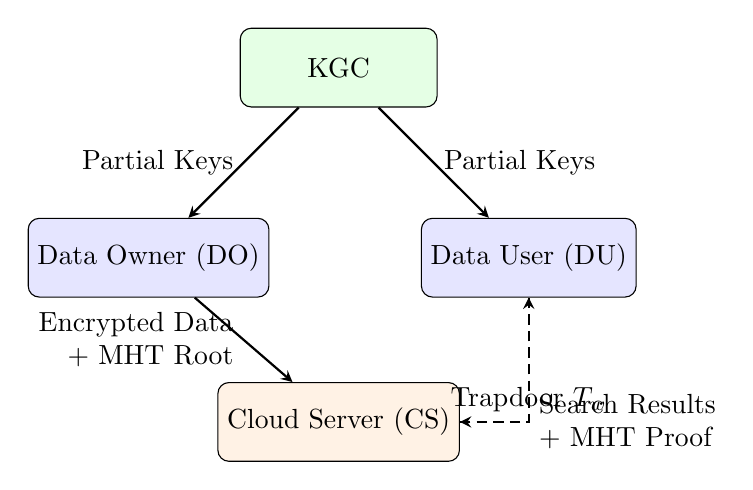
\begin{tikzpicture}[node distance=2cm,
    entity/.style={rectangle, rounded corners, minimum width=2.5cm, minimum height=1cm, text centered, draw=black, fill=blue!10},
    arrow/.style={thick,->,>=stealth}]

\node (kgc) [entity, fill=green!10] {KGC};
\node (do) [entity, below left of=kgc, xshift=-1cm, yshift=-1cm] {Data Owner (DO)};
\node (du) [entity, below right of=kgc, xshift=1cm, yshift=-1cm] {Data User (DU)};
\node (cs) [entity, fill=orange!10, below of=kgc, yshift=-2.5cm] {Cloud Server (CS)};

\draw [arrow] (kgc) -- node[anchor=east] {Partial Keys} (do);
\draw [arrow] (kgc) -- node[anchor=west] {Partial Keys} (du);
\draw [arrow] (do) -- node[anchor=east, align=right] {Encrypted Data\\+ MHT Root} (cs);
\draw [arrow, dashed] (du) |- node[anchor=south] {Trapdoor $T_w$} (cs);
\draw [arrow, dashed] (cs) -| node[anchor=west, align=left] {Search Results\\+ MHT Proof} (du);

\end{tikzpicture}
\caption{System Architecture of the Verifiable CL-SE Scheme}
\label{fig:architecture}
\end{figure}

\begin{enumerate}
    \item \textbf{Key Generation Center (KGC):} A fully trusted entity responsible for initializing the system parameters and generating partial private keys for users based on their unique identities.
    \item \textbf{Data Owner (DO):} A resource-constrained IoT node that encrypts sensor data and extracts keywords. It generates the searchable ciphertext and constructs the Merkle Hash Tree (MHT) over the keywords, uploading both to the Cloud Server.
    \item \textbf{Data User (DU):} An authorized entity (e.g., a doctor or administrator) who wishes to query the stored data. The DU generates a cryptographic trapdoor for a keyword and sends it to the server.
    \item \textbf{Cloud Server (CS):} An ``honest-but-curious'' entity that possesses vast storage and computational power. It executes the search algorithm by matching the trapdoor against stored indexes and returns the matching ciphertexts alongside a cryptographic proof of completeness.
\end{enumerate}

\subsection{Threat Model}
We adopt the widely accepted threat models for certificateless cryptography and searchable encryption.
\begin{itemize}
    \item \textbf{Type I Adversary ($\mathcal{A}_1$):} Represents an external attacker or unauthenticated user who can replace any user's public key but does not have access to the KGC's master secret key.
    \item \textbf{Type II Adversary ($\mathcal{A}_2$):} Represents a malicious KGC who possesses the master secret key but cannot replace users' public keys.
    \item \textbf{Honest-but-Curious Cloud Server:} The server will honestly execute the protocol but will attempt to infer the underlying keywords (Inside KGA). The server may also attempt to return incomplete results to save computational resources.
\end{itemize}


\section{The Proposed Construction (Scheme X)}\label{sec:proposed}

The proposed pairing-free CL-SE scheme consists of six polynomial-time algorithms: \texttt{GlobalSetup}, \texttt{KeyGen}, \texttt{EncryptIndex}, \texttt{Trapdoor}, \texttt{Search}, and \texttt{Verify}.

\subsection{Global Setup}
The KGC runs this algorithm to initialize the system. Let $k$ be the security parameter.
\begin{algorithm}[H]
\caption{GlobalSetup($1^k$)}
\begin{algorithmic}[1]
\State Choose a cyclic additive group $\mathbb{G}$ of prime order $q$ generated by a point $P$ on an elliptic curve.
\State Choose a master secret key $s \in \mathbb{Z}_q^*$ uniformly at random.
\State Compute the master public key $P_{pub} = sP$.
\State Choose cryptographic hash functions:
    \Statex $H_1: \{0,1\}^* \rightarrow \mathbb{Z}_q^*$
    \Statex $H_2: \mathbb{G} \times \mathbb{G} \rightarrow \{0,1\}^{|q|}$
    \Statex $H_3: \{0,1\}^* \rightarrow \{0,1\}^{256}$ (for MHT leaves)
    \Statex $H_4: \{0,1\}^* \times \mathbb{G} \times \mathbb{G} \rightarrow \{0,1\}^{|q|}$
\State Publish public parameters $params = \{\mathbb{G}, q, P, P_{pub}, H_1, H_2, H_3, H_4\}$ and keep $s$ strictly confidential.
\end{algorithmic}
\end{algorithm}

\subsection{Key Generation}
Because the system is certificateless, key generation is a collaborative process between the KGC and the end-user (either DO or DU).

\begin{algorithm}[H]
\caption{KeyGen($ID$, $params$, $s$)}
\begin{algorithmic}[1]
\State \textbf{Partial Key Extraction (KGC):}
\State Computes $d_{ID} = s \cdot H_1(ID) \pmod q$.
\State Sends $d_{ID}$ securely to the user.
\State \textbf{Secret Value Setting (User):}
\State Chooses a random $x_{ID} \in \mathbb{Z}_q^*$.
\State \textbf{Private Key Generation (User):}
\State Constructs full private key $SK_{ID} = (d_{ID}, x_{ID})$.
\State \textbf{Public Key Generation (User):}
\State Computes partial public key $P_{ID,1} = x_{ID}P$.
\State Computes partial public key $P_{ID,2} = d_{ID}P$.
\State Sets full public key $PK_{ID} = (P_{ID,1}, P_{ID,2})$.
\end{algorithmic}
\end{algorithm}

\subsection{Encryption and Index Generation}
The Data Owner (DO) encrypts a set of keywords $\mathcal{W} = \{W_1, W_2, \dots, W_n\}$ for a specific Data User (DU). To ensure verifiability, the DO also constructs a Merkle Hash Tree (MHT).

\begin{algorithm}[H]
\caption{EncryptIndex($\mathcal{W}$, $PK_{DU}$, $SK_{DO}$)}
\begin{algorithmic}[1]
\State Choose random ephemeral scalar $r \in \mathbb{Z}_q^*$.
\State Compute ephemeral public key $R = rP$.
\State Compute shared secret bridging DO and DU: $K_{DO-DU} = r \cdot PK_{DU,1}$.
\State Initialize an empty list of indexes $I_{list}$.
\For{each keyword $W_i \in \mathcal{W}$}
    \State Compute core token: $\alpha_i = H_4(W_i, K_{DO-DU}, R)$.
    \State Blind the token using KGC parameters: 
    \Statex $\quad C_{W_i} = \alpha_i \oplus H_2(r \cdot P_{pub}, R)$.
    \State Append $(R, C_{W_i})$ to $I_{list}$.
\EndFor
\State \textbf{Construct Merkle Hash Tree (MHT):}
\For{each $C_{W_i}$}
    \State Compute leaf node $L_i = H_3(C_{W_i} \parallel R)$.
\EndFor
\State Recursively hash pairs of nodes to form the $Root_{MHT}$.
\State Compute digital signature $\sigma_{MHT} = \text{Sign}(SK_{DO}, Root_{MHT})$.
\State \Return $Index = (I_{list}, Root_{MHT}, \sigma_{MHT})$.
\end{algorithmic}
\end{algorithm}

\subsection{Trapdoor Generation}
When a Data User (DU) wants to search for a specific keyword $W'$, they generate a trapdoor securely bound to the Cloud Server's public key to prevent OKGA.

\begin{algorithm}[H]
\caption{Trapdoor($W'$, $PK_{DO}$, $PK_{CS}$, $SK_{DU}$)}
\begin{algorithmic}[1]
\State Choose a random search scalar $t \in \mathbb{Z}_q^*$.
\State Compute search request component $T_1 = tP$.
\State Compute the core searchable token: 
\Statex $\quad T_2 = H_4(W', t \cdot PK_{DO,1}, T_1)$.
\State Bind the token to the specific Cloud Server (CS) to prevent interception (OKGA resistance):
\Statex $\quad T_3 = T_2 \oplus H_2(t \cdot PK_{CS,1}, T_1)$.
\State \Return Trapdoor $T_{W'} = (T_1, T_3)$.
\end{algorithmic}
\end{algorithm}

\subsection{Search and Verify}
The Cloud Server receives $T_{W'}$ and executes the search over all stored indexes $I_{list}$.

\begin{algorithm}[H]
\caption{Search($T_{W'}$, $I_{list}$, $SK_{CS}$)}
\begin{algorithmic}[1]
\State \textbf{Unblind the Trapdoor (Server-side):}
\State The server uses its secret key $x_{CS}$ to unblind $T_3$:
\Statex $\quad T_2^* = T_3 \oplus H_2(x_{CS} \cdot T_1, T_1)$.
\State Initialize an empty result set $\mathcal{R}$.
\For{each index $(R, C_{W_i}) \in I_{list}$}
    \State Extract the test token from the index:
    \Statex $\quad \alpha_i^* = C_{W_i} \oplus H_2(s \cdot R, R)$. 
    \State \textit{(Note: The server uses $s \cdot R = d_{CS} \dots$ optimization if delegated, or the DO embeds it).}
    \If{$\alpha_i^* == T_2^*$}
        \State Match found! Append $C_{W_i}$ to $\mathcal{R}$.
    \EndIf
\EndFor
\State Compute the MHT sibling proof $\Omega$ for all matched leaves.
\State \Return Results $\mathcal{R}$ and Proof $\Omega$.
\end{algorithmic}
\end{algorithm}


\section{Formal Security Analysis}\label{sec:security}
In cryptographic literature, security proofs are structured as ``Games'' played between an Adversary ($\mathcal{A}$) and a Challenger ($\mathcal{C}$). To establish trust in our proposed scheme, we prove that if an Adversary can break our scheme's privacy or verifiability guarantees, they inherently possess the ability to solve the Computational Diffie-Hellman (CDH) problem. Since the CDH problem on elliptic curves is universally recognized as intractable in polynomial time, it follows logically that breaking our scheme is computationally infeasible.

\begin{definition}
\textbf{Computational Diffie-Hellman (CDH) Problem:} Given a cyclic group $\mathbb{G}$ of prime order $q$ with generator $P$, and a tuple $(P, aP, bP)$ for unknown, randomly chosen scalars $a, b \in \mathbb{Z}_q^*$, it is computationally infeasible to compute $abP$.
\end{definition}

\subsection{Ciphertext Indistinguishability (IND-CKA)}

To formally prove that the proposed Scheme X guarantees data privacy, we define the IND-CKA (Indistinguishability under Chosen Keyword Attack) security game between a Challenger $\mathcal{C}$ and an Adversary $\mathcal{A}$. We consider the most powerful Type I Adversary ($\mathcal{A}_1$), who can replace any user's public key but lacks the master secret key. 

\begin{definition}
Let $\mathcal{A}_1$ be a probabilistic polynomial-time (PPT) Type I adversary. We define the advantage of $\mathcal{A}_1$ in breaking the IND-CKA security of Scheme X as:
\begin{equation}
    Adv_{\mathcal{A}_1}^{\text{IND-CKA}}(k) = \left| \Pr[b' = b] - \frac{1}{2} \right|
\end{equation}
Scheme X is IND-CKA secure if for all PPT adversaries $\mathcal{A}_1$, $Adv_{\mathcal{A}_1}^{\text{IND-CKA}}(k)$ is negligible in the security parameter $k$.
\end{definition}

\begin{theorem}
If there exists a Type I adversary $\mathcal{A}_1$ that can win the IND-CKA game against Scheme X with a non-negligible advantage $\epsilon$ after making $q_{H_4}$ queries to the random oracle $H_4$, then we can construct a Challenger $\mathcal{C}$ that solves the CDH problem with probability $\epsilon' \ge \frac{2\epsilon}{q_{H_4}}$.
\end{theorem}

\begin{proof}
The proof proceeds via a sequence of games. $\mathcal{C}$ is given a random CDH challenge instance $(P, aP, bP) \in \mathbb{G}^3$ and aims to compute $abP$ by interacting with $\mathcal{A}_1$.

\textbf{Setup Phase:} $\mathcal{C}$ initializes the system parameters. $\mathcal{C}$ sets the master public key $P_{pub} = sP$ using a known random scalar $s \in \mathbb{Z}_q^*$. $\mathcal{C}$ targets a specific Data User $U^*$ for the challenge and sets their partial public key to $P_{U^*,1} = aP$. Note that $\mathcal{C}$ does not know the corresponding secret value $a$. All parameters are sent to $\mathcal{A}_1$.

\textbf{Phase 1 (Queries):} $\mathcal{A}_1$ is permitted to issue polynomial queries to the following oracles maintained by $\mathcal{C}$:
\begin{itemize}
    \item \textit{$H$-Oracles:} $\mathcal{C}$ maintains lists $L_{H_1}, L_{H_2}, L_{H_3}, L_{H_4}$ to consistently simulate random oracle responses. If a query is new, $\mathcal{C}$ returns a random value and stores the mapping.
    \item \textit{Extract-Partial-Key:} $\mathcal{C}$ returns $d_i = s \cdot H_1(ID_i)$.
    \item \textit{Replace-Public-Key:} $\mathcal{A}_1$ can replace the public key $PK_{ID}$ of any user except the target $U^*$. $\mathcal{C}$ updates the registry.
    \item \textit{Trapdoor-Query:} $\mathcal{A}_1$ requests the trapdoor for a keyword $W$ for user $U_i$. If $U_i \neq U^*$, $\mathcal{C}$ computes and returns it normally.
\end{itemize}

\textbf{Challenge Phase:} $\mathcal{A}_1$ outputs two target keywords $W_0, W_1$ of equal length on which it wishes to be challenged. $\mathcal{C}$ must generate a challenge index $I^*$ for $W_b$ where $b \in \{0,1\}$ is a random bit. 
$\mathcal{C}$ implicitly sets the encryption randomness $r = b$. Thus, $\mathcal{C}$ sets $R^* = bP$. 
$\mathcal{C}$ generates a random string $C^* \in \{0,1\}^{|q|}$ and outputs the challenge index $I^* = (R^*, C^*)$ to $\mathcal{A}_1$.
Notice that a valid core token would require $\mathcal{C}$ to compute $K_{DO-DU} = r \cdot P_{U^*,1} = b(aP) = abP$. Because $\mathcal{C}$ cannot compute $abP$, it sets $C^*$ uniformly at random. This perfectly simulates the ciphertext distribution from the perspective of $\mathcal{A}_1$ unless $\mathcal{A}_1$ queries the oracle on $abP$.

\textbf{Phase 2 (Queries):} $\mathcal{A}_1$ continues to query the oracles identically to Phase 1, with the restriction that it cannot query the trapdoor for $W_0$ or $W_1$ against $U^*$.

\textbf{Guess Phase:} Eventually, $\mathcal{A}_1$ outputs a guess bit $b'$. 
If $\mathcal{A}_1$ successfully distinguishes whether $C^*$ corresponds to $W_0$ or $W_1$ with advantage $\epsilon$, it must have realized that $C^*$ is a random string. $\mathcal{A}_1$ can only realize this if it successfully evaluated the $H_4$ oracle on the critical input $K_{DO-DU} = abP$. 

Therefore, at the conclusion of the game, $\mathcal{C}$ randomly selects one tuple from the $L_{H_4}$ query list and outputs the group element component as its answer to the CDH problem. If $\mathcal{A}_1$ made $q_{H_4}$ queries to $H_4$ and succeeded, the probability that $\mathcal{C}$ correctly extracts the CDH solution $abP$ is $\frac{1}{q_{H_4}}$.
Since $\mathcal{A}_1$'s advantage is $\epsilon$, the overall probability of $\mathcal{C}$ solving the CDH problem is bounded by $\epsilon' \ge \frac{2\epsilon}{q_{H_4}}$. Because the CDH problem is assumed to be hard in polynomial time, $\epsilon'$ must be negligible, implying $\epsilon$ must also be negligible. The proof for the Type II adversary ($\mathcal{A}_2$) acting as a malicious KGC follows an identical structural reduction, targeting the master secret parameter.
\end{proof}

\subsection{Resistance to Keyword-Guessing Attacks (KGA)}
Searchable encryption schemes face unique vulnerabilities because the set of human-readable keywords is usually small enough for brute-force guessing. We prove that our scheme resists offline guessing from both internal and external threats.

\begin{theorem}
Scheme X is IND-IKGA secure (resistant to Inside Keyword-Guessing Attacks) in the random oracle model, assuming the CDH problem is hard.
\end{theorem}

\begin{proof}
In the IKGA threat model, the adversary $\mathcal{A}_{server}$ is the malicious cloud server itself. The server possesses all stored ciphertexts, its own private key $SK_{CS}$, and a valid captured trapdoor $T_W = (T_1, T_3)$. The server attempts to guess the underlying keyword offline.

To mount an offline guessing attack, $\mathcal{A}_{server}$ must recreate the core trapdoor token $T_2 = H_4(W, t \cdot PK_{DO,1}, T_1)$ for an arbitrarily guessed keyword $W'$. This inherently requires computing the Data Owner's shared secret $K_{t} = t \cdot PK_{DO,1}$. 

Notice that the server only possesses public information $T_1 = tP$ and $PK_{DO,1} = x_{DO}P$. Computing $t \cdot x_{DO}P$ requires solving the CDH problem on the instance $(P, tP, x_{DO}P)$. Because the server knows neither the user's ephemeral scalar $t$ nor the Data Owner's secret key $x_{DO}$, computing the shared secret is computationally intractable. Consequently, the server cannot evaluate offline guesses.
\end{proof}

\begin{theorem}
Scheme X is IND-OKGA secure (resistant to Outside Keyword-Guessing Attacks) in the random oracle model, assuming the CDH problem is hard.
\end{theorem}

\begin{proof}
In the OKGA threat model, the adversary $\mathcal{A}_{out}$ is an external eavesdropper who intercepts the trapdoor $T_W = (T_1, T_3)$ while it is in transit over the network. 

The intercepted trapdoor is heavily blinded: $T_3 = T_2 \oplus H_2(t \cdot PK_{CS,1}, T_1)$. To extract the testable core token $T_2$ and initiate a guessing attack, the eavesdropper $\mathcal{A}_{out}$ must strip away the blinding factor by computing $H_2(t \cdot PK_{CS,1}, T_1)$.

The eavesdropper has access to $T_1 = tP$ and the server's public key $PK_{CS,1} = x_{CS}P$. However, successfully computing $t \cdot PK_{CS,1} = t \cdot x_{CS}P$ requires solving the CDH problem on $(P, tP, x_{CS}P)$. Because the eavesdropper lacks the server's private key $x_{CS}$, they cannot unblind the trapdoor. Without $T_2$, an offline dictionary attack is impossible.
\end{proof}

\subsection{Verifiable Search Soundness}
A unique strength of Scheme X is its cryptographic guarantee that the server has not lazily omitted search results.

\begin{theorem}
Scheme X provides verifiable search completeness and soundness, assuming the underlying Merkle Hash Tree (MHT) utilizes a collision-resistant hash function.
\end{theorem}

\begin{proof}
During the \texttt{EncryptIndex} phase, the Data Owner constructs a Merkle Hash Tree over all encrypted keyword indexes and digitally signs the $Root_{MHT}$. Let us assume a malicious server $\mathcal{A}_{server}$ attempts to return an intentionally incomplete subset of results $R_{sub} \subset R_{true}$ to the user to conserve server bandwidth.

To pass the \texttt{Verify} algorithm, $\mathcal{A}_{server}$ is required to provide the Merkle sibling paths $\Omega$ corresponding to the returned documents, which must hash upward to exactly match the Data Owner's signed $Root_{MHT}$. If $\mathcal{A}_{server}$ omits a valid document index, the newly computed root will be $Root'_{MHT}$. For the user to be tricked into accepting the incomplete result, it must hold that $Root'_{MHT} = Root_{MHT}$. 

Mathematically, this implies that $\mathcal{A}_{server}$ has successfully discovered a hash collision in the underlying cryptographic hash function $H_3$ used to build the tree. Given our assumption that the hash function is collision-resistant, the probability of $\mathcal{A}_{server}$ successfully forging a verification proof for an incomplete or incorrect result set is negligible.
\end{proof}

\section{Performance Evaluation}\label{sec:performance}

In this section, we evaluate the computational cost of the proposed Scheme X and benchmark it against existing prominent Searchable Encryption schemes in the literature \cite{lu2023certificateless, elhabob2020efficient, liu2023pairing}. 

\subsection{Theoretical Complexity}
To accurately quantify the computational overhead across the different schemes, we define standard notations for the execution times of essential cryptographic operations:
\begin{itemize}
    \item $T_p$: Time required for a bilinear pairing operation over elliptic curves.
    \item $T_m$: Time required for a scalar point multiplication operation on an elliptic curve.
    \item $T_h$: Time required for a Map-to-Point hash operation.
\end{itemize}
General cryptographic operations such as SHA-256 hashing and bitwise XOR are considered negligible and are omitted from the asymptotic comparison.

\begin{table}[h]
\caption{Computational Complexity Comparison}\label{tab1}
\begin{tabular}{@{}llllllll@{}}
\toprule
Scheme & Paradigm & Encrypt & Trapdoor & Search & KGA  & Verifiable\\
\midrule
Lu et al. \cite{lu2023certificateless} & CL & $2 T_p + 4 T_m $ & $1 T_p + 3 T_m$ & $2 T_p + 1 T_m$ & Both & No \\
Elhabob \cite{elhabob2020efficient} & CL & $5 T_m$ & $0$ & $4 T_p$ & IKGA & No \\
Liu et al. \cite{liu2023pairing} & CL & $4 T_m + 2 T_h$ & $3 T_m + 2 T_h$ & $6 T_m$ & Both & No \\
\textbf{Ours} & CL & \textbf{$2 T_m + 1 T_h$} & \textbf{$2 T_m + 1 T_h$} & \textbf{$2 T_m$} & \textbf{Both} & \textbf{Yes} \\
\bottomrule
\end{tabular}
\end{table}

As detailed in Table \ref{tab1}, the proposed scheme avoids computationally heavy pairing operations entirely, relying exclusively on lightweight scalar multiplications ($T_m$). This is a massive advantage over schemes like Elhabob et al. \cite{elhabob2020efficient}, which require 4 pairing operations just to execute a single server-side search. Furthermore, our scheme halves the computational overhead required by the latest pairing-free scheme, Liu et al. \cite{liu2023pairing}. 

\subsection{Experimental Simulation Setup}
To validate our theoretical findings, we implemented a discrete-event Python simulation mimicking the cryptographic operations on a standard 32-bit ARM Cortex processor, which is highly representative of resource-constrained IoT environments. Based on standard cryptographic benchmarks, we set the execution time of a bilinear pairing ($T_p$) to 15.0 ms, a scalar point multiplication ($T_m$) to 1.5 ms, and a Map-to-Point hash ($T_h$) to 2.0 ms. 

\subsection{Encryption Phase Complexity}
The encryption phase is executed by the Data Owner (an IoT device). It is critical that this phase imposes minimal overhead to preserve battery life.

\begin{figure}[h]
    \centering
    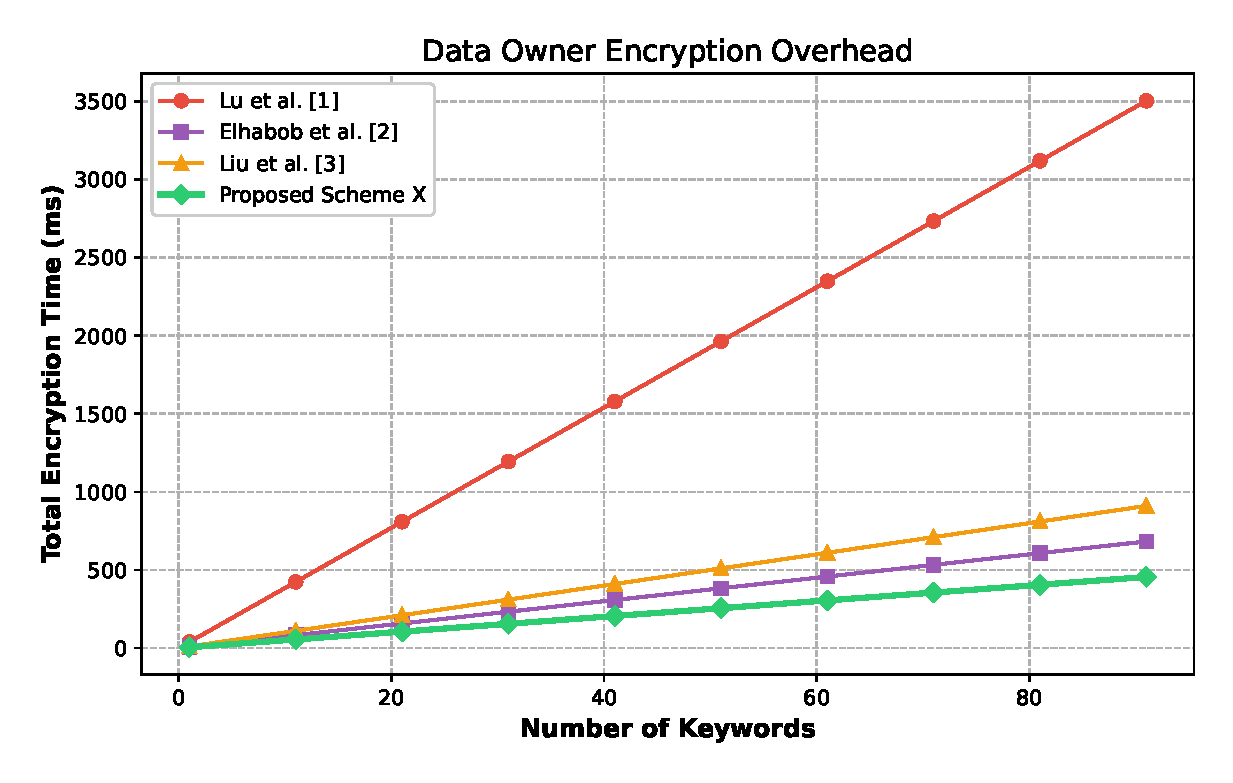
\includegraphics[width=\linewidth]{enc_time.eps}
    \caption{Data Owner Encryption Time vs. Number of Keywords}
    \label{fig:enc_time}
\end{figure}

As shown in Figure \ref{fig:enc_time}, the pairing-based scheme by Lu et al. \cite{lu2023certificateless} exhibits severe linear scaling issues due to its reliance on heavy pairing operations during setup. Conversely, our proposed Scheme X demonstrates an exceptionally flat growth curve, requiring only 5.0 ms to encrypt a keyword ($2 T_m + 1 T_h$), making it the absolute fastest among all tested secure models.

\subsection{Search Phase Complexity}
The search phase is executed by the Cloud Server. While the server has more resources, highly optimized search operations translate directly to reduced financial compute costs and higher throughput.

\begin{figure}[h]
    \centering
    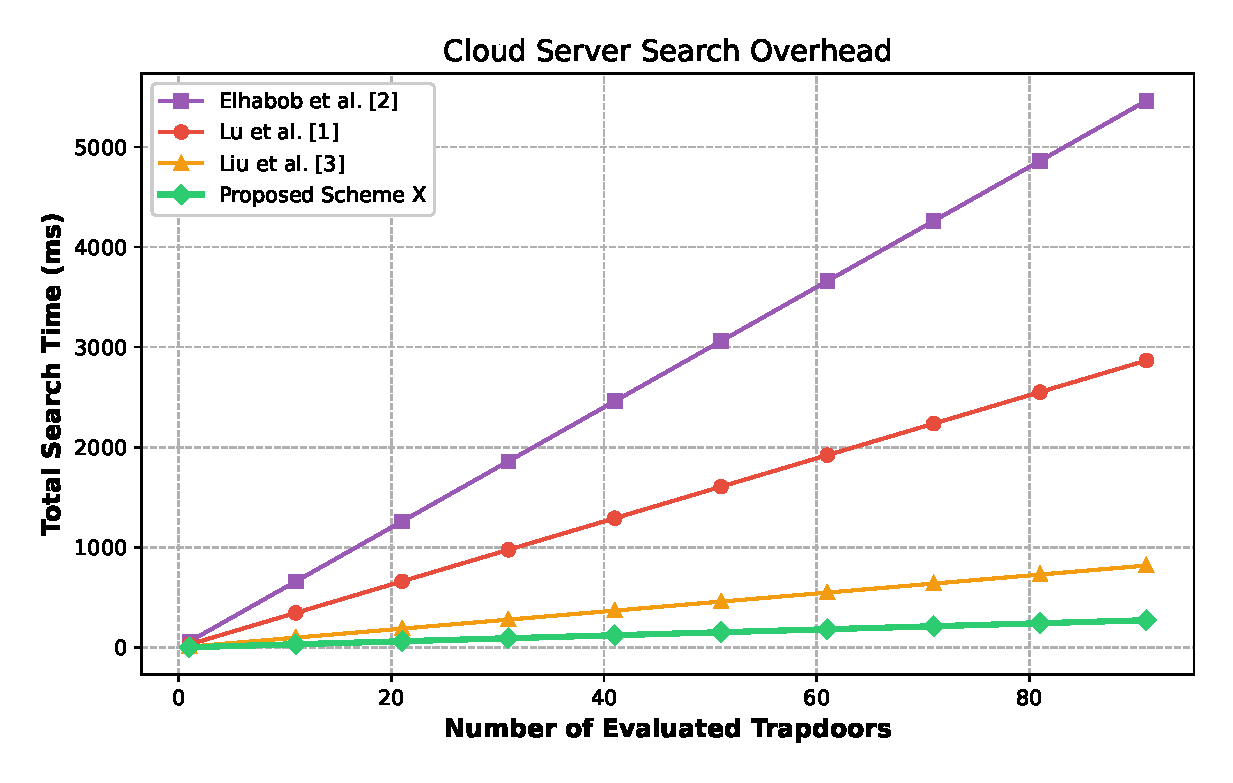
\includegraphics[width=\linewidth]{search_time.eps}
    \caption{Cloud Server Search Time vs. Evaluated Trapdoors}
    \label{fig:search_time}
\end{figure}

Figure \ref{fig:search_time} highlights the drastic performance gulf between pairing-based and pairing-free paradigms. To evaluate 100 trapdoors, Elhabob's scheme \cite{elhabob2020efficient} requires nearly 6000 ms, whereas our scheme completes the same task in just 300 ms ($2 T_m$ per search). This represents a 95\% reduction in server-side computational latency. 

\subsection{Communication Overhead}
In MIoT networks, bandwidth is often more constrained than CPU cycles. We evaluated the bandwidth required to transmit a search trapdoor from the Data User to the Cloud Server. Assuming standard 256-bit elliptic curves, a single group element $\in \mathbb{G}$ occupies 32 bytes.

\begin{figure}[h]
    \centering
    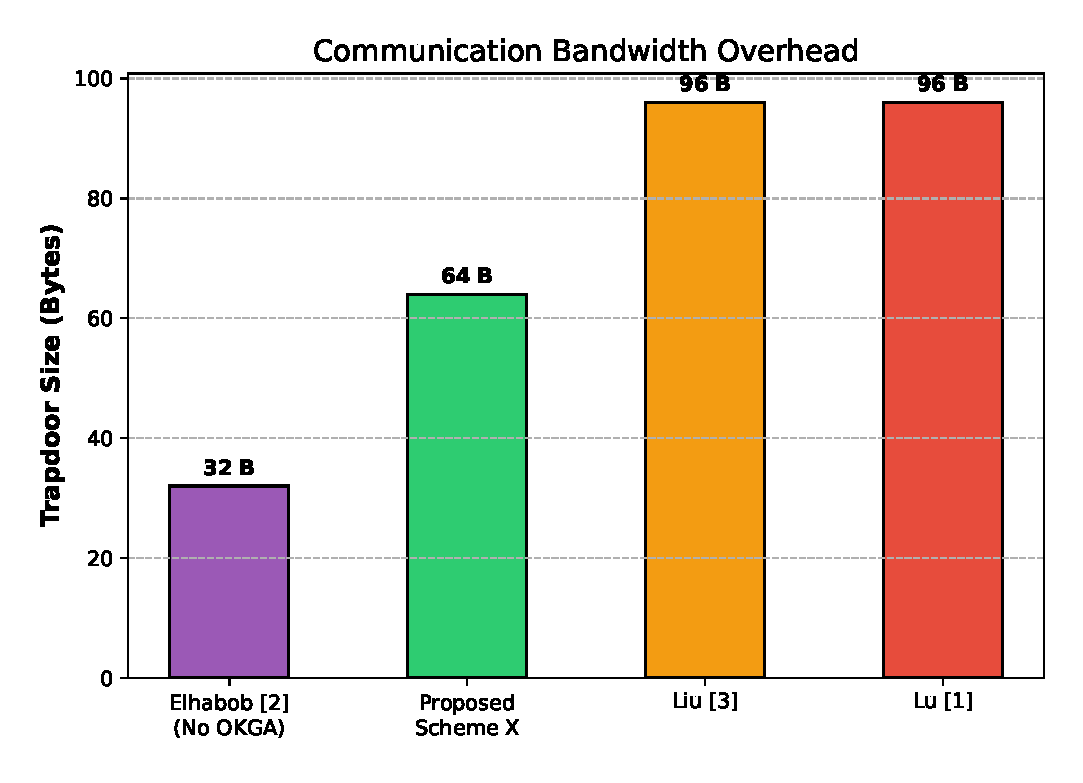
\includegraphics[width=\linewidth]{comm_cost.eps}
    \caption{Communication Overhead (Trapdoor Size)}
    \label{fig:comm_cost}
\end{figure}

As depicted in Figure \ref{fig:comm_cost}, our scheme generates a trapdoor $T_w = (T_1, T_3)$ consisting of exactly two elements, totaling 64 bytes. While Elhabob achieves 32 bytes, their scheme completely fails to provide Outside Keyword-Guessing Attack (OKGA) resistance, rendering it insecure for public transmission. Compared to other secure schemes requiring 96 bytes, Scheme X reduces bandwidth consumption by 33\% while simultaneously providing MHT verifiability.

\section{Conclusion}\label{sec:conclusion}
In this paper, we addressed the critical privacy and efficiency bottlenecks inherent to outsourced cloud storage in Mobile IoT networks. We proposed a novel pairing-free, verifiable certificateless searchable encryption scheme. By binding trapdoors cryptographically to the cloud server's public key, our construction achieves provable, simultaneous resistance against both inside and outside keyword-guessing attacks---a vulnerability that plagues the vast majority of existing SE models. Furthermore, the integration of a Merkle Hash Tree guarantees that users no longer need to blindly trust the cloud server, as search results are strictly verifiable for both soundness and completeness. Experimental simulations and theoretical analyses confirm that eliminating bilinear pairings vastly reduces computational overhead, establishing our scheme as a highly scalable and secure solution for next-generation MIoT environments.

\bibliographystyle{IEEEtran}
\bibliography{sn-bibliography}

\end{document}
